\subsection{多次元配列}

内部的には、多次元配列は本質的には一次元の配列と同じです。

コンピュータメモリは一次元なので、メモリは一次元配列です。
便宜上、多次元配列は一次元として表現可能です。

例えば、3x4の配列の要素が12のセルの1次元配列にどのように配置されるかを示します。

% TODO FIXME not clear. First, horizontal would be better. Second, why two columns?
% I'd first show 3x4 with numbered elements (e.g. 32-bit ints) in colored lines,
% then linear with the same numbered elements (and colored blocks)
% then linear with addresses (offsets) - assuming let say 32-bit ints.
\begin{table}[H]
\centering
\begin{tabular}{ | l | l | }
\hline
Offset in memory & array element \\
\hline
0 & [0][0] \\
\hline
1 & [0][1] \\
\hline
2 & [0][2] \\
\hline
3 & [0][3] \\
\hline
4 & [1][0] \\
\hline
5 & [1][1] \\
\hline
6 & [1][2] \\
\hline
7 & [1][3] \\
\hline
8 & [2][0] \\
\hline
9 & [2][1] \\
\hline
10 & [2][2] \\
\hline
11 & [2][3] \\
\hline
\end{tabular}
\caption{1次元配列としてメモリ上で表現される2次元配列}
\end{table}

3*4配列の各セルがメモリ上でどう配置されるかを示します。

% TODO coordinates. TikZ?
\begin{table}[H]
\centering
\begin{tabular}{ | l | l | l | l | }
\hline                        
0 & 1 & 2 & 3 \\
\hline  
4 & 5 & 6 & 7 \\
\hline  
8 & 9 & 10 & 11 \\
\hline  
\end{tabular}
\caption{2次元配列の各セルのメモリアドレス}
\end{table}

\myindex{row-major order}

したがって、必要な要素のアドレスを計算するには、まず最初のインデックスに
4(配列の幅)を掛けてから2番目のインデックスを追加します。
これは\emph{行優先順位}と呼ばれ、配列と行列表現のこの方法は、少なくとも \CCpp とPythonで使用されます。
単純な英単語の\emph{行優先順位}は、\q{最初に、最初の行の要素を書き、次に2番目の行 \dots 
最後に最後の行の要素を書き込む}という意味です。

\myindex{column-major order}
\myindex{Fortran}
表現のもう1つの方法は、\emph{列優先順位}(配列の添字は逆順で使用されます)と呼ばれ、
少なくともFortran、MATLAB、およびRで使用されます。
\emph{列優先順位}は、単純な英語では、\q{最初に、最初の列の要素を書き込み、次に2番目の列を \dots
最後に最後の列の要素を書き込む}となります。

どの方法が良いでしょうか?

一般に、パフォーマンスとキャッシュメモリの観点からは、
データ編成のための最良の方法は、要素が順次アクセスされる方法です。

したがって、関数が行ごとにデータにアクセスする場合は、\emph{行優先順位}が優れていて、逆もまた同様です。

% subsubsections
\subsubsection{2次元配列の例}

\Tchar 型の配列で作業していきます。これは、各要素がメモリ上に1バイトしか必要ないことを意味します。

\myparagraph{行を埋める例}
\myindex{\olly}

2行目を0~3の値で埋めてみましょう。

\lstinputlisting[caption=行を埋める例,style=customc]{patterns/13_arrays/5_multidimensional/two1_JA.c}

3つの行はすべて赤でマークしてあります。
2行目は0,1,2と3の値を持っています。

\begin{figure}[H]
\centering
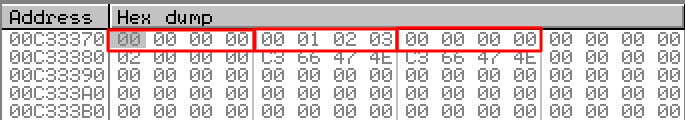
\includegraphics[width=0.6\textwidth]{patterns/13_arrays/5_multidimensional/olly_2D_1.png}
\caption{\olly: 配列が埋められる}
\end{figure}

\myparagraph{列を埋める例}
\myindex{\olly}

3列目を値0~2で埋めてみましょう。

\lstinputlisting[caption=列を埋める例,style=customc]{patterns/13_arrays/5_multidimensional/two2_JA.c}

3つの行はここでも赤でマークしてあります。

各行の3番目の値が0,1と2で書かれています。

\begin{figure}[H]
\centering
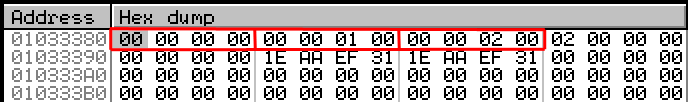
\includegraphics[width=0.6\textwidth]{patterns/13_arrays/5_multidimensional/olly_2D_2.png}
\caption{\olly: 配列が埋められる}
\end{figure}


\subsubsection{2次元配列を1次元配列としてアクセスする}

少なくとも2つの方法で、2次元配列を1次元配列としてアクセスすることが可能だといえます。

\lstinputlisting[style=customc]{patterns/13_arrays/5_multidimensional/2D_as_1D_JA.c}

コンパイルして実行してください。\footnote{プログラムはC++ではなく、Cプログラムとしてコンパイルされます。.c拡張子でファイルを保存してMSVCでコンパイルします}
正しい値を表示します。

MSVC 2013の結果は興味部会です。3つのルーチンはすべて同じです!

\lstinputlisting[caption=\Optimizing MSVC 2013 x64,style=customasmx86]{patterns/13_arrays/5_multidimensional/2D_as_1D_MSVC_2013_Ox_x64_JA.asm}

GCCも同じルーチンを生成しますが、少し異なります。

\lstinputlisting[caption=\Optimizing GCC 4.9 x64,style=customasmx86]{patterns/13_arrays/5_multidimensional/2D_as_1D_GCC49_x64_O3_JA.s}


\subsubsection{3次元配列の例}

多次元配列でも同じです。

\Tint 型の配列で作業していきます。各要素はメモリ上で4バイト必要とします。

見てみましょう。

\lstinputlisting[caption=単純な例,style=customc]{patterns/13_arrays/5_multidimensional/multi.c}

\myparagraph{x86}

MSVC 2010の結果

\lstinputlisting[caption=MSVC 2010,style=customasmx86]{patterns/13_arrays/5_multidimensional/multi_msvc_JA.asm}

特別なことはありません。インデックスの計算では、式 $address=600 \cdot 4 \cdot x + 30 \cdot 4 \cdot y + 4z$ 
では3つの入力引数が使用され、配列を多次元として表現しています。
\Tint 型は32ビット(4バイト)なので、
係数は4倍する必要があることを忘れないでください。

\lstinputlisting[caption=GCC 4.4.1,style=customasmx86]{patterns/13_arrays/5_multidimensional/multi_gcc_JA.asm}

GCCコンパイラは異なります。

計算での演算において($30y$)、GCCは乗算命令を使わないコードを生成します。
このようにします。
$(y+y) \ll 4 - (y+y) = (2y) \ll 4 - 2y = 2 \cdot 16 \cdot y - 2y = 32y - 2y = 30y$. 
従って、 $30y$ の計算には、加算命令が1つだけです。
ビットシフト演算と減算が使用されます。
これはより高速です。

\myparagraph{ARM + \NonOptimizingXcodeIV (\ThumbMode)}

\lstinputlisting[caption=\NonOptimizingXcodeIV (\ThumbMode),style=customasmARM]{patterns/13_arrays/5_multidimensional/multi_Xcode_thumb_O0_JA.asm}

\NonOptimizing LLVMは変数すべてをローカルスタックに保存しますが、冗長です。

配列の要素のアドレスはすでに見た式によって計算されます。

\myparagraph{ARM + \OptimizingXcodeIV (\ThumbMode)}

\lstinputlisting[caption=\OptimizingXcodeIV (\ThumbMode),style=customasmARM]{patterns/13_arrays/5_multidimensional/multi_Xcode_thumb_O3_JA.asm}

既に見たシフト、加減算による乗算を置き換えるためのトリックもここにあります。

\myindex{ARM!\Instructions!RSB}
\myindex{ARM!\Instructions!SUB}
新しい命令を見てみます:\RSB (\emph{Reverse Subtract})

単純に \SUB として機能しますが、実行前にオペランドをスワップします。
なぜでしょう?
\myindex{ARM!Optional operators!LSL}
\SUB および \RSB は、シフト係数が適用される第2のオペランド(\INS{LSL\#4})への命令です。

ただし、この係数は第2オペランドにのみ適用されます。

これは、加算や乗算のような可換的な(交換可能な)演算の場合は問題ありません。
(結果を変更せずにオペランドを入れ替えてもかまいません)

しかし、減算は非可換的な演算なので、 \RSB が存在します。

\myparagraph{MIPS}

\myindex{MIPS!Global Pointer}
私の例はとても小さいので、GCCコンパイラはグローバルポインタによってアドレス可能な64KiB領域に
配列を配置することに決めました。

\lstinputlisting[caption=\Optimizing GCC 4.4.5 (IDA),style=customasmMIPS]{patterns/13_arrays/5_multidimensional/multi_MIPS_O3_IDA_JA.lst}


%\input{patterns/13_arrays/5_multidimensional/dimensions_JA}

\subsubsection{More examples}

コンピュータ画面は2D配列として表現されますが、ビデオバッファは1次元配列です。
これについてはこちらで:\myref{Mandelbrot_demo}

本書での他の例としてはマインスイーパーゲームがあります。そのフィールドは2次元配列です:\myref{minesweeper_winxp}
